% % % % % % % % % % % % % % 
%
%	U.S. Chartbook
%	Brian W. Dew (brianwdew@gmail.com)
%	Updated: November 5, 2023
%	GitHub repo contains to do list (issues)
%   https://github.com/bdecon/US-chartbook
%
% % % % % % % % % % % % % %
\PassOptionsToPackage{table}{xcolor}
\documentclass{report}

%
% % % % % % Packages % % % % % % % % % 
%
	
	\usepackage[letterpaper, margin=1.0in]{geometry}
	\usepackage{microtype}
	\usepackage[default]{lato}
	\usepackage{pgfplots, pgfplotstable}
	\usepackage[eulergreek]{sansmath}
	\usepackage{amssymb}
	\usepackage{xcolor}
	\definecolor{usaablue}{RGB}{18,57,91}
	\usepackage{array}
	\usepackage{fontawesome5}
	\usepackage{imakeidx}
	\usepackage{titlesec}
	\usepackage{fancyhdr}
	\usepackage{enumitem}
	\usepackage{float}
	\usepackage{wrapfig}
\usepackage{caption}
\captionsetup{labelformat=empty}

\def\debug{1}
	\usepackage{environ}

	
	\usepackage[colorlinks, linkcolor=blue, filecolor=blue, 
		citecolor=blue, urlcolor=blue, linktoc=all, 
		pdfencoding=auto]{hyperref}
	\usetikzlibrary{pgfplots.dateplot, pgfplots.fillbetween, patterns,
	                pgfplots.groupplots, shapes.geometric}

%
% % % % % Document Settings % % % % % % % 
%

	% Paragraph spacing
	\usepackage{parskip}
	\setlength\parindent{0pt}
	\setlength{\parskip}{8pt}
	\makeatletter
		\newcommand{\@minipagerestore}{\setlength{\parskip}{8pt}}
	\makeatother
	
% Section and Subsection Headings
	\titleformat{\section}
  		{\color{usaablue} \LARGE \seriffont \bfseries}
  		{\thesection}{1em}{}
	\titleformat{\subsection}
  		{\color{usaablue} \seriffont \bfseries \large}
  		{\thesection}{1em}{}
	\titleformat{\subsubsection}
  		{\color{usaablue} \seriffont \bfseries \normalsize}
  		{\thesection}{1em}{}		
	

  	% References remove numbering
	\makeatletter
		\renewcommand\@biblabel[1]{}
	\makeatother
%
% % % % % Graph Settings % % % % % % % 
%
	% Custom page style for section pages
	\fancypagestyle{sectpage}{\fancyhf{}\renewcommand{\headrulewidth}{0pt}
		\fancyhead[R]{\textcolor{blue!70}{\rule[-0.5pt]{4pt}{6pt}} \hspace{-1.5mm}
		\textcolor{green!70!blue}{\rule[-0.5pt]{4pt}{9pt}} \color{black!90} 
			\seriffont US Chartbook}
		\lfoot{\footnotesize Updated: \today}
		\rfoot{\hyperlink{toc}{\faList}}
		\cfoot{\thepage}}
		
	% Header and footer
	
	\pagestyle{fancy}
	\fancyhf{}
	\renewcommand{\headrulewidth}{0pt}
	\rfoot{\color{usaablue}\thepage}
	\cfoot{\color{usaablue}CONFIDENTIAL}

	
	
	% Index
	\indexsetup{level=\section*,noclearpage}
	\makeindex
	
	% Color square
	\newcommand{\cbox}[1]{
		\begin{tikzpicture} \draw [#1, line width=6](0,0) -- (.2,0);  
		\end{tikzpicture}}
	\newcommand{\bcbox}[1]{
		\begin{tikzpicture}[overlay]\draw [#1, line width=9](-0.25,0.22) -- (-3.0,0.22);  
		\end{tikzpicture}}
	\newcommand{\colorline}[2]{
		\begin{tikzpicture} \draw [#1, line width=1.8](0,0.2) -- +(0.6,0) 
			node[right, black!80] {#2}; 
		\end{tikzpicture}}
	\newcommand{\colordashline}[2]{
		\begin{tikzpicture} \draw [densely dashed, #1, line width=1.8](0,0.2) -- +(0.5,0) 
			node[right, black!80] {#2}; 
		\end{tikzpicture}}
	\newcommand{\scolorline}[2]{
		\begin{tikzpicture} \draw [#1, line width=2.0](0,0.2) -- +(0.3,0) 
			node[right, black!80] {#2}; 
		\end{tikzpicture}}
		
	% Table link
	\newcommand{\tbllink}[1]{\href{https://raw.githubusercontent.com/bdecon/US-chartbook/master/chartbook/data/#1}{\faTable}}
	
	% Table of Contents entry
	\newcommand{\tocentry}[2]{\item \seriffont {#2}
		 \  \  \  \  \  \footnotesize \hyperlink{#1}{\textit{\pageref*{#1}}} \normalsize}
	\newcommand{\tocentsm}[2]{\item \small {#2}
		 \  \  \  \  \  \footnotesize \hyperlink{#1}{\textit{\pageref*{#1}}} \normalsize}
	
	% Last two digits of year
	\makeatletter
	\newcommand*\short[1]{\expandafter\@gobbletwo\number\numexpr#1\relax}
	\makeatother	
	
	% Column width and alignment
	\newcolumntype{R}[1]{>{\raggedleft\let\newline\\\arraybackslash\hspace{0pt}}m{#1}}	
	\newcolumntype{C}[1]{>{\centering\let\newline\\\arraybackslash\hspace{0pt}}m{#1}}
	
	% Style for date plots
	\pgfplotsset{compat=newest, 
		scaled y ticks=false,
		axis line style={black!20}, 
		xtick style={black!20}, ytick style={draw=none},
		every tick label/.style={black!50, font=\scriptsize,
			/pgf/number format/assume math mode=true},
		width=12cm, height=6cm, 
		xticklabel style={align=left}, 
		yticklabel style={text width=0.9em, align=right},       
		axis x line*=bottom, x axis line style={black!50},
	    axis y line=left, y axis line style={opacity=0},
	    ymajorgrids, grid style={very thin, black!10},	        
	    every node near coord/.style={/pgf/number format/fixed,
	    	font=\scriptsize, style={black!70}},
	    legend style={legend columns=-1, draw=none, fill=none,
	    	/tikz/every even column/.append style={column sep=0.3cm}}}
	    	
	
	% stacked diverging bar
	\newcommand{\sbar}[4]{
		\addplot[ybar stacked, bar width=2.3pt, draw opacity=0, fill=#1] 
			table [x=#2, y=#3, col sep=comma]{#4};}

	% stacked diverging bar area legend
	\newcommand{\sbaral}[4]{
		\addplot[ybar stacked, bar width=2.3pt, draw opacity=0, fill=#1, area legend] 
			table [x=#2, y=#3, col sep=comma]{#4};}
			
	% thin stacked diverging bar
	\newcommand{\tsbar}[4]{
		\addplot[ybar stacked, bar width=2.1pt, draw opacity=0, fill=#1] 
			table [x=#2, y=#3, col sep=comma]{#4};}
			
	% custom width stacked diverging bar
	\newcommand{\ctsbar}[5]{
		\addplot[ybar stacked, bar width=#5, draw opacity=0, fill=#1] 
			table [x=#2, y=#3, col sep=comma]{#4};}
			
	% area plot segment
	\newcommand{\abar}[4]{
		\addplot[stack plots=y, area style, draw=none, fill=#1] 
			table [x=#2, y=#3, col sep=comma]{#4}\closedcycle;}
					
	% text node
	\newcommand{\stdnode}[3]{\node[below, align=left, shift=({#1,#2})]{#3};}	
	
	% text node located by data	 
	\newcommand{\absnode}[3]{\node[below right, align=left] at (axis cs: #1,#2) {#3};}   
	
	% multiline text node located by data	 
	\newcommand{\absnodeml}[4]{\node[below right, align=left, text width=#4cm] 
		at (axis cs: #1,#2) {#3};}       
		        
	% Date (X) Axis Tick Marks, one tick per year, every even year labeled
	\newcommand{\dateaxisticks}{
		date coordinates in=x, axis line style={draw=none},
		xmax={2024-01-31},
		max space between ticks=40,	    
		xtick={{1990-01-01}, {1992-01-01}, {1994-01-01}, 
			{1996-01-01}, {1998-01-01}, {2000-01-01}, 
			{2002-01-01}, {2004-01-01}, {2006-01-01},
			{2008-01-01}, {2010-01-01}, {2012-01-01}, {2014-01-01},
		    {2016-01-01}, {2018-01-01}, {2020-01-01}, {2022-01-01}, 
		    {2024-01-01}, {2026-01-01}},
		minor xtick={{1989-01-01}, {1991-01-01}, {1993-01-01},
			{1995-01-01}, {1997-01-01}, {1999-01-01}, 
			{2001-01-01}, {2003-01-01}, {2005-01-01}, {2007-01-01},
		    {2009-01-01}, {2011-01-01}, {2013-01-01}, {2015-01-01},
		    {2017-01-01}, {2019-01-01}, {2021-01-01}, {2023-01-01}, 
		    {2025-01-01}, {2027-01-01}},
		enlarge y limits={0.06}, enlarge x limits={0.01},
		xticklabel style={align=center, yshift=-2pt}, tick label style={inner sep=0pt},
		}
		
	% Date (X) Axis Tick Marks, one tick per year, every even year labeled
	\newcommand{\shdateaxisticks}{
		date coordinates in=x, axis line style={draw=none},
		xmax={2024-01-31},
		max space between ticks=40,	    
		xtick={{1990-01-01}, {1995-01-01}, {2000-01-01}, 
			{2005-01-01}, {2010-01-01}, {2015-01-01}, {2020-01-01}},
		minor xtick={},
		enlarge y limits={0.06}, enlarge x limits={0.01},
		xticklabel style={align=center, yshift=-2pt}, tick label style={inner sep=0pt},
		}
		
	% Date (X) Axis Tick Marks, one tick per year, every even year labeled
	\newcommand{\ltdateaxisticks}{
		date coordinates in=x, axis line style={draw=none},
		xmax={2024-01-31},
		max space between ticks=40,	    
		xtick={{2013-01-01}, {2014-01-01}, {2015-01-01}, {2016-01-01}, 
			{2017-01-01}, {2018-01-01}, {2019-01-01}, {2020-01-01}, {2021-01-01},
			{2022-01-01}, {2023-01-01}, {2024-01-01}},
		enlarge y limits={0.06}, enlarge x limits={0.01},
		xticklabel style={align=center, yshift=-2pt}, tick label style={inner sep=0pt},
		}
		
	% Date (X) Axis Tick Marks, one tick per year, every even year labeled
	\newcommand{\lfdateaxisticks}{
		date coordinates in=x, axis line style={draw=none},
		xmin={2018-01-01}, xmax={2024-01-31},   
		xtick={{2018-01-01}, {2019-01-01}, {2020-01-01}, {2021-01-01}, 
			{2022-01-01}, {2023-01-01}, {2024-01-01}},
		enlarge y limits={value=0.12, upper}, enlarge x limits={0.02}, ymin=0,
		yticklabel style={text width=1.0em},
		height=3.8cm, width=6.4cm,
		}
		
	% Date (X) Axis Tick Marks, one tick per year, every even year labeled
	\newcommand{\tydateaxisticks}{
		date coordinates in=x, axis line style={draw=none},
		xmax={2024-01-31}, max space between ticks=40,	    
		xtick={{2011-01-01}, {2012-01-01}, {2013-01-01}, {2014-01-01}, {2015-01-01},
		 {2016-01-01}, {2017-01-01}, {2018-01-01}, {2019-01-01}, {2020-01-01}, 
		 {2021-01-01}, {2022-01-01}, {2023-01-01}, {2024-01-01}},
		enlarge y limits={0.06}, enlarge x limits={0.01},
		}
		
	% Date (X) Axis Tick Marks, very short term monthly ticks
	\newcommand{\shticks}{
		date coordinates in=x, axis line style={draw=none},
		xmax={2024-01-31},
		}

	% Date (X) Axis Tick Marks, no tick marks, just formatting
	\newcommand{\empticks}{
		date coordinates in=x, axis line style={draw=none},
		xticklabels=\empty, xtick style={draw=none},
		xmax={2024-01-31}, enlarge x limits={0.01},
		}
		
	% Settings for y label text in horizontal bar charts
	\newcommand{\barylab}[2]{yticklabel style={text width=#1, align=right, 
		style={black!70}, text height=#2},}
	
	% Solid bars at significant  x or y values
	\newcommand{\bbar}[2]{extra #1 ticks = {{#2}}, extra #1 tick labels = ,
		extra #1 tick style = {grid=major, grid style={thick, black!25}},}
		
	% Dashed line at significant  x or y values
	\newcommand{\dbar}[2]{extra #1 ticks = {{#2}}, extra #1 tick labels = ,
		extra #1 tick style = {grid=major, grid style={dashed, thick, black!50}},}
		
	% Standard line
	\newcommand{\stdline}[4]{\addplot[very thick, no markers, color=#1] 
		table [x=#2, y=#3, col sep=comma] {#4};	}
		
	% Thin line
	\newcommand{\thinline}[4]{\addplot[no markers, color=#1] 
		table [x=#2, y=#3, col sep=comma] {#4};	}
		
	% Dashed line
	\newcommand{\dashline}[4]{\addplot[very thick, densely dashed, no markers, color=#1] 
		table [x=#2, y=#3, col sep=comma] {#4};	}
		
	% Thicker line
	\newcommand{\thickline}[4]{\addplot[ultra thick, no markers, color=#1] 
		table [x=#2, y=#3, col sep=comma] {#4};	}
		
	% Style for bar plots legend symbol		
	\pgfplotsset{/pgfplots/area legend/.style={/pgfplots/legend image code/.code={
		\fill[##1] (0cm, -0.1cm) rectangle (0.6cm, 0.1cm);}},}		
		
	% Additional bar plot settings
	\newcommand{\barplotnogrid}{xbar=0pt, axis line style={draw=none},
	    yticklabel style={align=left, anchor=east},
      		xmajorticks=false, ymajorgrids=false,   
	    ytick=data, tickwidth=0pt, area legend, reverse legend,
	    nodes near coords align={horizontal},}  
		
	% Recession bars		
	\newcommand{\rbars}{
		\fill[color=black!10] (axis cs:{1990-07-01},\pgfkeysvalueof{/pgfplots/ymin})
			rectangle (axis cs:{1991-03-01}, \pgfkeysvalueof{/pgfplots/ymax});
		\fill[color=black!10] (axis cs:{2007-12-01},\pgfkeysvalueof{/pgfplots/ymin})
			rectangle (axis cs:{2009-07-01}, \pgfkeysvalueof{/pgfplots/ymax});
		\fill[color=black!10] (axis cs:{2001-03-01},\pgfkeysvalueof{/pgfplots/ymin})
			rectangle (axis cs:{2001-11-01}, \pgfkeysvalueof{/pgfplots/ymax});
		\fill[color=black!10] (axis cs:{2020-02-01},\pgfkeysvalueof{/pgfplots/ymin})
			rectangle (axis cs:{2020-05-01}, \pgfkeysvalueof{/pgfplots/ymax});}
			
	\newcommand{\rebars}{
		\fill[color=black!10] (axis cs:{2007-12-01},\pgfkeysvalueof{/pgfplots/ymin}) 
			rectangle (axis cs:{2009-07-01}, \pgfkeysvalueof{/pgfplots/ymax});
		\fill[color=black!10] (axis cs:{2001-03-01},\pgfkeysvalueof{/pgfplots/ymin}) 
			rectangle (axis cs:{2001-11-01}, \pgfkeysvalueof{/pgfplots/ymax});
		\fill[color=black!10] (axis cs:{2020-02-01},\pgfkeysvalueof{/pgfplots/ymin}) 
			rectangle (axis cs:{2020-05-01}, \pgfkeysvalueof{/pgfplots/ymax});}
			
	\newcommand{\recbars}{
		\fill[color=black!10] (axis cs:{2007-12-01},\pgfkeysvalueof{/pgfplots/ymin})
			rectangle (axis cs:{2009-07-01}, \pgfkeysvalueof{/pgfplots/ymax});
		\fill[color=black!10] (axis cs:{2020-02-01},\pgfkeysvalueof{/pgfplots/ymin}) 
			rectangle (axis cs:{2020-05-01}, \pgfkeysvalueof{/pgfplots/ymax});}
			
	\newcommand{\rbar}{
		\fill[color=black!10] (axis cs:{2020-02-01},\pgfkeysvalueof{/pgfplots/ymin}) 
			rectangle (axis cs:{2020-05-01}, \pgfkeysvalueof{/pgfplots/ymax});}
	
	\newfontfamily\seriffont{RobotoSlab}	
	
	\pgfplotstableread[header=true, col sep=comma]{data/unempgroups.csv}\unemp
	\pgfplotstableread[header=true, col sep=comma]{data/unempgroups2.csv}\unempt
	\pgfplotstableread[header=true, col sep=comma]{data/unempgroups3.csv}\unemptt
	\pgfplotstableread[header=true, col sep=comma]{data/cpi_monthly.csv}\cpimo
	\pgfplotstableread[header=true, col sep=comma]{data/gdp_rec2.csv}\gdprecs
	\pgfplotstableread[header=true, col sep=comma]{data/lprod_rec.csv}\lprodrec	
	\pgfplotstableread[header=true, col sep=comma]{data/pa_epop_rec.csv}\paepoprec
	\pgfplotstableread[header=true, col sep=comma]{data/ahe_monthly.csv}\ahemo	
	
	
% % % % % % % %
%
%  Begin Document
%
% % % % % % % %		
\begin{document}
\setlength\intextsep{0pt}
\setlength{\columnsep}{8pt}
\setlength{\wrapoverhang}{0pt}


\chapter*{
		\includegraphics{blue_eagle.png}\\\color{usaablue} Blue Book}
\vspace*{-16mm}

\footnotesize %\hspace{11mm} 
\color{usaablue}v0.2, \today \normalsize 

\vspace{11mm}

\normalsize \color{usaablue}CFO Overview of Macro Economy, USAA Financials, and Member Health

\vspace{16mm}

\thispagestyle{empty}

\begin{minipage}{0.36\textwidth}
\subsection*{ {\color{red} \faExclamationTriangle} \seriffont Notes}

{\color{red} \textbf{Initial draft:}} \\
Content is draft form. \\ Not to be circulated 
\vfill

\end{minipage}
\begin{minipage}{0.36\textwidth}
\subsection*{{\color{gray} \faUser} Contact}

\textbf{Enterprise Modeling} \  \\
{\color{gray} \faEnvelope} \ edward.blackburne@usaa.com \ \\

\end{minipage}


\newcommand\BB{{\color{usaablue}Blue Book}}
\begin{minipage}{1.0\textwidth}
\subsection*{About the \BB}
\color{black}
The USAA \BB\  is a collection of notes describing economic and social developments in the United States since 1989. The notes are grouped into sections, each covering one macroeconomic sector or one major aspect of the economy. Each section contains charts, tables, descriptive text, and links to relevant materials. 

The Blue Book is kept up to date by connecting to public data sources. The latest version of the chartbook is located at \href{https://www.bd-econ.com/chartbook.html}{uschartbook.com}, and the \href{https://github.com/bdecon/US-chartbook}{source code} is available on GitHub. 

Ultimately, the chartbook aims to be useful for macroeconomic analysis, to inspire researchers and students, and to facilitate research and exploration.
\end{minipage}
\newpage
\thispagestyle{sectpage}
\subsection*{Key Economic Indicators}

\begin{minipage}{1.0\textwidth}
\small The following six charts summarize recent economic developments. Each topic: output, prices, productivity, employment, wage growth, and job growth, is covered in more depth in the chartbook. Click the chart icon \normalsize {\color{blue}\faChartBar[regular]} \small to go to the relevant chartbook section.
\end{minipage}
\vspace{1mm}

\begin{minipage}{0.3\textwidth}
\normalsize \textbf{Real GDP Growth} \ \hyperlink{gdpgr}{\faChartBar[regular]}\\
\footnotesize{\textit{seasonally-adjusted annual rate}}
\vspace{2.35cm}

\hspace{2mm} \begin{tikzpicture}[overlay]
	\begin{axis}[ybar=24pt, \bbar{y}{0}, date coordinates in=x, 
    	xtick=data,	xticklabels from table={\gdprecs}{Quarter},
		clip=false, height=4.45cm, width=5.8cm, 
		enlarge y limits={0.28}, enlarge x limits={0.06},
		minor xtick={{2022-01-01}, {2023-01-01}, {2024-01-01}, {2025-01-01}},
		xticklabel style={align=center, yshift=-2pt}, minor tick length=7pt, 
		tick label style={inner sep=0pt}, xticklabel pos=lower,
		yticklabel style={text width=1.0em}, 
		visualization depends on=abs(\thisrow{A191RL})/\thisrow{A191RL}*4 \as \myshift,
    	every node near coord/.append style = {yshift={\myshift}},
		axis line style={draw=none}, nodes near coords,
		nodes near coords style={/pgf/number format/.cd, fixed zerofill,
			precision=1, assume math mode}]
	%\input{text/gdp_rec2_bar_node.txt}
	\ctsbar{red!90!black}{date}{A191RL}{\gdprecs}{11pt}
	\node[align=left] at (rel axis cs:0.95, 1.02) {\color{black!55!white}\footnotesize {\textit{Est.}}};
	\input{text/gdpnow_node.txt}
	\end{axis}
\end{tikzpicture} 
\end{minipage}\hspace{6mm} \begin{minipage}{0.3\textwidth}
\vfill 
\normalsize \textbf{Consumer Price Index} \ \hyperlink{cpimm}{\faChartBar[regular]}\\
\footnotesize{\textit{percent change from previous month}}
\vspace{2.6cm}

\hspace{2mm} \begin{tikzpicture}[overlay]
	\begin{axis}[\bbar{y}{0}, date coordinates in=x, axis line style={draw=none},
		enlarge y limits={0.24}, enlarge x limits={0.02}, 
		width=5.7cm, height=4.7cm, tick label style={inner sep=0pt},
		yticklabel style={text width=1.2em}, clip=false, xtick=data,
		xticklabels from table={\cpimo}{label2},
		minor xtick={{2022-01-01}, {2023-01-01}, {2024-01-01}, {2025-01-01}},
		xticklabel style={align=center}, minor tick length=7pt]
	%\input{text/cpi_rec_bar_node.txt}
	\addplot[thick, draw opacity=0] table [x=date, y=FILL, col sep=comma]{\cpimo};
	\addplot[ybar, fill=blue!90!black, bar width=4.0pt, draw opacity=0] table 
	[x=date, y=ALL_S, col sep=comma]{\cpimo};
	\draw [black!30!white, dashed] (rel axis cs:0.35,0) -- 
		(rel axis cs:0.35, 0.99);
	\node[below right, align=left] at (rel axis cs:0.35, 1.0) {\color{black!55!white}\footnotesize {latest 12 months}};
	\draw [black!30!white, dashed] (rel axis cs:0.96,0) -- 
		(rel axis cs:0.96, 0.9);
	\node[align=left] at (rel axis cs:0.995, 0.92) {\color{black!65!white}\footnotesize {\textit{Est.}}};
	\input{text/cpinow_node2.txt}
	\end{axis}
\end{tikzpicture}
\end{minipage} \hspace{4mm} \begin{minipage}{0.3\textwidth}
\normalsize \textbf{Productivity Growth} \ \hyperlink{lprodgr}{\faChartBar[regular]}\\
\footnotesize{\textit{total economy, annual rate}}
\vspace{2.35cm}

\hspace{3mm} \begin{tikzpicture}[overlay]
	\begin{axis}[ybar=24pt, \bbar{y}{0}, date coordinates in=x, 
    	xtick=data,	xticklabels from table={\lprodrec}{Quarter},
		clip=false, height=4.45cm, width=5.8cm, ymax=6,
		enlarge y limits={0.28}, enlarge x limits={0.06},
		minor xtick={{2022-01-01}, {2023-01-01}, {2024-01-01}, {2025-01-01}},
		xticklabel style={align=center, yshift=-2pt}, minor tick length=7pt, 
		tick label style={inner sep=0pt}, xticklabel pos=lower,
		yticklabel style={text width=1.0em}, 
		visualization depends on=abs(\thisrow{LPROD_gr})/\thisrow{LPROD_gr}*4 \as \myshift,
    	every node near coord/.append style = {yshift={\myshift}},
		axis line style={draw=none}, nodes near coords,
		nodes near coords style={/pgf/number format/.cd, fixed zerofill,
			precision=1, assume math mode}]
	%\input{text/lprod_rec_bar_node.txt}
	\ctsbar{cyan!70!white}{date}{LPROD_gr}{\lprodrec}{11pt}
	\node[align=left] at (rel axis cs:0.95, 1.02) {\color{black!55!white}\footnotesize {\textit{Est.}}};
	\draw [black!30!white, dashed] (rel axis cs:0.89,0) -- 
		(rel axis cs:0.89, 0.99);
	\input{text/lprod_rec_node.txt}
	\end{axis}
\end{tikzpicture}
\end{minipage}
\vspace{4mm}

\begin{minipage}{0.3\textwidth}
\vfill

\normalsize \textbf{Employment Rate} \ \hyperlink{epoplt}{\faChartBar[regular]}\\
\footnotesize{\textit{age 25 to 54, percent}}
\vspace{2.6cm}

\hspace{2mm} \begin{tikzpicture}[overlay]
	\begin{axis}[\bbar{y}{0}, \shticks 
		xtick=data, clip=false,  date coordinates in=x,
		enlarge x limits={0.05}, tick label style={inner sep=0pt},
		enlarge y limits={0.3}, yticklabel style={text width=1.2em}, 
		height=4.7cm, width=5.7cm, 
		minor xtick={{2022-01-01}, {2023-01-01}, {2024-01-01}, {2025-01-01}},
		xticklabel style={align=center}, minor tick length=7pt, 
		xticklabels from table={\paepoprec}{label}, ]
	\stdline{green!50!black}{date}{PA_EPOP_M}{\paepoprec}
	\thickline{blue!80!purple}{date}{PA_EPOP}{\paepoprec}
	\stdline{yellow!40!orange}{date}{PA_EPOP_W}{\paepoprec}
	\input{text/epop_summary_nodes.txt}
	\stdline{cyan}{date}{PA_EPOP}{\paepoprec}
	\end{axis}
\end{tikzpicture} 
\end{minipage}\hspace{6mm} \begin{minipage}{0.3\textwidth}
\vfill 
\normalsize \textbf{Average Hourly Earnings} \ \hyperlink{ahelt}{\faChartBar[regular]}\\
\footnotesize{\textit{percent change from previous month}}
\vspace{2.6cm}

\hspace{1mm} \begin{tikzpicture}[overlay]
	\begin{axis}[\bbar{y}{0}, date coordinates in=x, axis line style={draw=none},
		enlarge y limits={0.36}, enlarge x limits={0.02}, 
		width=5.7cm, height=4.7cm, tick label style={inner sep=0pt},
		yticklabel style={text width=1.6em}, clip=false, xtick=data,
		legend cell align={left},
		legend style={legend columns=-1, at={(rel axis cs:0.99, 0.21)}},
		xticklabels from table={\ahemo}{label},
		minor xtick={{2022-01-01}, {2023-01-01}, {2024-01-01}, {2025-01-01}},
		xticklabel style={align=center}, minor tick length=7pt]
%	\input{text/cpi_rec_bar_node.txt}
	\addplot[thick, draw opacity=0] table [x=date, y=FILL, col sep=comma]{\ahemo};
	\addplot[only marks, mark=square*, fill=violet!90!black, mark size=2.2pt, 
		draw opacity=0] table 
	[x=date, y=ALL, col sep=comma]{\ahemo};
	\addplot[only marks, mark=diamond*, fill=white, draw=magenta, mark size=2.0pt] table 
	[x=date, y=REAL, col sep=comma]{\ahemo};
	\draw [black!30!white, dashed] (rel axis cs:0.35,0) -- 
		(rel axis cs:0.35, 0.99);
	\node[below right, align=left] at (rel axis cs:0.35, 1.0) {\color{black!55!white}\footnotesize {latest 12 months}};
	\legend{, Nominal, Real};
	\draw [black!40!white, fill=white] (rel axis cs:0.37, 0.05) rectangle (rel axis cs:0.97, 0.2);
	\input{text/ahe_summary_nodes.txt}
	\end{axis}
\end{tikzpicture}
\end{minipage} \hspace{5mm} \begin{minipage}{0.3\textwidth}
\vfill 
\normalsize \textbf{Private Nonfarm Payrolls} \ \hyperlink{nfplt}{\faChartBar[regular]}\\
\footnotesize{\textit{change from previous month, thousands}}
\vspace{2.6cm}

\hspace{4mm} \begin{tikzpicture}[overlay]
	\begin{axis}[\bbar{y}{0}, date coordinates in=x, 
    	xtick=data,	xticklabels from table={\ahemo}{label},
		clip=false, height=4.65cm, width=5.5cm, 
		enlarge y limits={0.18}, enlarge x limits={0.03},
		minor xtick={{2022-01-01}, {2023-01-01}, {2024-01-01}, {2025-01-01}},
		xticklabel style={align=center, yshift=-2pt}, minor tick length=7pt, 
		tick label style={inner sep=0pt}, xticklabel pos=lower,
		yticklabel style={text width=2.2em}, 
		axis line style={draw=none}]
	\addplot[thick, draw opacity=0] table [x=date, y=FILL, col sep=comma]{data/nfp_monthly.csv};
	\ctsbar{orange!92!red}{date}{NFP}{data/nfp_monthly.csv}{4pt}
	\input{text/nfp_summary_node.txt}
	\end{axis}
\end{tikzpicture}
\end{minipage}
\newpage
\section*{\hyperlink{toc}{\faList} \ {Contents}}
\thispagestyle{sectpage}
\hypertarget{toc}{}
\vspace{3mm}
\normalsize

\hspace*{-3mm}\begin{minipage}[t]{0.45\textwidth}
\setlength{\parskip}{2.4pt}
\begin{description}
\tocentry{oea}{\cbox{gray} Overall Economic Activity}
\begin{description}[labelindent=-2mm]
\tocentsm{oety}{Types of Activity}
\tocentsm{oegr}{Economic Growth}
\tocentsm{oegc}{Components of Growth}
\end{description}
\vspace{3mm}

\tocentry{ofa}{\cbox{lightgray} Overall Financial Activity}
\begin{description}[labelindent=-2mm]
\tocentsm{ofl}{Liabilities}
\tocentsm{ofsb}{Sectoral Balances}
\tocentsm{ofw}{Wealth}
\tocentsm{ofi}{Investment}
\end{description}
\vspace{3mm}

\tocentry{hh}{\cbox{red!90!black} Households}
\begin{description}[labelindent=-2mm]
\tocentsm{hhdem}{Demographics}
\tocentsm{hhinc}{Income}
\tocentsm{hhss}{Spending and Saving}
\tocentsm{hhbs}{Balance Sheets}
\tocentsm{hhh}{Housing}
\tocentsm{hhpov}{Poverty}
\end{description}
\vspace{3mm}

\tocentry{bus}{\cbox{blue!90!white} Businesses}
\begin{description}[labelindent=-2mm]
\tocentsm{busin}{Investment}
\tocentsm{buspr}{Corporate Profits}
\tocentsm{busbs}{Balance Sheets}
\tocentsm{busip}{Industrial Production}
\tocentsm{busrs}{Retail Sales}
\end{description}
\vspace{3mm}

\tocentry{gov}{\cbox{green!80!blue} Government}
\begin{description}[labelindent=-2mm]
\tocentsm{govce}{Current Economic Activity}
\tocentsm{govco}{Contribution to Growth}
\tocentsm{govre}{Receipts and Expenditures}
\tocentsm{govjo}{Government Jobs}
\tocentsm{govbs}{Balance Sheets}
\end{description}
\vspace{3mm}

\tocentry{ext}{\cbox{violet} External Sector}
\begin{description}[labelindent=-2mm]
\tocentsm{exbop}{Balance of Payments}
\tocentsm{extt}{International Trade}
\tocentsm{exiip}{International Investment}
\tocentsm{excf}{Capital Flows}
\tocentsm{extfx}{Exchange Rates}
\end{description}
\end{description}
\end{minipage} \hspace{2mm} 
\begin{minipage}[t]{0.48\textwidth}
\setlength{\parskip}{2.4pt}
\begin{description}
\tocentry{lab}{\cbox{cyan} Labor Markets}
\begin{description}[labelindent=-2mm]
\tocentsm{labe}{Employment}
\tocentsm{labu}{Unemployment}
\tocentsm{labp}{Participation}
\tocentsm{labf}{Labor Force Flows}
\tocentsm{labh}{Hours}
\tocentsm{labns}{Nonstandard Arrangements}
\tocentsm{labw}{Wages}
\tocentsm{labprod}{Productivity}
\tocentsm{labun}{Union Membership}
\end{description}
\vspace{3mm}

\tocentry{cap}{\cbox{orange!80!yellow} Capital Markets}
\begin{description}[labelindent=-2mm]
\tocentsm{capeq}{Equity Markets}
\tocentsm{capint}{Interest Rates}
\tocentsm{capmm}{Money and Monetary Policy}
\end{description}
\vspace{3mm}

\tocentry{pr}{\cbox{purple!60!magenta} Prices}
\begin{description}[labelindent=-2mm]
\tocentsm{prin}{Consumer Price Index}
\tocentsm{prie}{Inflation Expectations}
\tocentsm{prpce}{PCE Price Index}
\tocentsm{prp}{Producer Prices}
\tocentsm{prex}{Import and Export Prices}
\tocentsm{prco}{Commodities}
\end{description}
\vspace{3mm}

\tocentry{references}{References}

\tocentry{index}{Index}
\end{description}
\end{minipage}

\vfill
\hspace{11.4cm} \footnotesize Return to Table of Contents
    \begin{tikzpicture}[overlay]
        \draw (0,0.1) -- (0.4,-0.7);
    \end{tikzpicture}
\newpage
\vspace*{-12mm}

\section*{\bcbox{gray}Overall Economic Activity}
%\thispagestyle{sectpage}
%\begin{minipage}[t]{0.62\textwidth}

%\end{minipage}\hfill
\begin{wrapfigure}{r}{0.50\textwidth}
%\begin{minipage}[t]{0.35\textwidth}
\raggedright{\normalsize \textbf{GDP per capita}\\\footnotesize{\textit{in thousands of \input{text/gdp_ltdt.txt}dollars}}}
%\fbox{%
\begin{tikzpicture}
    \begin{axis}[\shdateaxisticks clip=false, 
    	yticklabel style={text width=1.0em},width=0.50\textwidth,
        xticklabel={`\short{\year}}, enlarge x limits={0.02}]
    \rbars
    \stdline{red!95!black}{date}{value}{data/gdppc.csv}
	\input{text/gdp_pc_node.txt}
    \end{axis}
%    (current bounding box.south west) rectangle
 %     (current bounding box.north east)
\end{tikzpicture}
\\\footnotesize{Source: Bureau of Economic Analysis}
%}
%\end{minipage}
\end{wrapfigure}\small
This analysis of the United States economy begins with the most popular measure of overall economic activity, \href{https://www.bea.gov/data/gdp/gross-domestic-product}{gross domestic product} (GDP). \hypertarget{oea}{\label{oea}}
\index{gross domestic product!overview}
\index{gross domestic product!per capita}
GDP is the value of goods and services produced in the US in a given time period. According to the Bureau of Economic Analysis, the seasonally-adjusted annualized US GDP was 
\if\debug1{\marginpar{\color{green}text/gdp1.txt}}\fi
\input{text/gdp1.txt}
\if\debug1{\marginpar{\color{red}text/gdp1.txt}}\fi

GDP calculated using the expenditures approach is the sum of major types of domestic spending on finished goods and services: consumer spending, private investment, and government spending and investment. To capture only domestic production, foreign spending on US produced goods and services is added, while imports (spending on non-US-produced goods and services) are subtracted.

\normalsize \textbf{Expenditures, by Type}\\
\footnotesize{\textit{per capita, seasonally-adjusted annualized rate, \input{text/gdp_ltdt.txt}dollars}}\\
\hspace*{-2mm} \rowcolors{1}{}{black!5} \setlength{\tabcolsep}{2.4pt} \color{black!90}
		{\renewcommand{\arraystretch}{1.54}
		% \begin{tabular}{p{48mm} R{12mm} R{12mm} R{12mm} R{12mm} R{12mm}}
		\begin{tabular}{lrrrrr} 			\input data/gdppc_levels.tex \hline
		\end{tabular}} \vspace{-2mm}
		
\footnotesize{Source: Bureau of Economic Analysis}
\newpage
\markright{\footnotesize \color{gray}{\rule[0.5pt]{6.5pt}{6.5pt}} \color{black!90} \normalsize  \seriffont \ Overall Economic Activity}
\vspace*{-8mm}

\end{document}
